\chapter{Avaliação Experimental} \label{Cap:AvaliacaoExperimental}

\FloatBarrier
\section{Análise Exploratória dos Dados} \label{sec:eda}

A análise exploratória revelou padrões comportamentais consistentes com a literatura de churn em e-commerce de varejo \cite{matuszelanski2022}. A distribuição de recência demonstra que clientes Ativos situam-se majoritariamente nos primeiros cem dias desde a última compra (66\% dos casos), com média de 84 dias, enquanto clientes Churn apresentam distribuição mais dispersa, com média de 126 dias e ocorrências isoladas que ultrapassam 400 dias de ausência. Essa separação confirma a recência, uma das dimensões centrais do framework RFM \cite{hughes1994}, como variável com poder discriminativo relevante.

A análise de frequência, segunda dimensão do RFM, evidencia que ambas as classes apresentam mediana de dois pedidos, mínimo imposto pelo filtro adotado, mas os clientes Ativos exibem média superior (2,56 contra 2,08 pedidos), com maior dispersão e valores extremos de até oito pedidos, contra seis entre os Churn. O review score médio apresenta diferença marginal entre as classes (Ativos: 4,25; Churn: 4,21), sugerindo que a satisfação declarada não é fator determinante isolado para a retenção, indicação de que o churn configura-se como um problema de engajamento, e não de qualidade do serviço \cite{manzoor2024}.

O perfil comparativo multivariado confirma que as dimensões mais discriminativas entre Ativos e Churn são o valor monetário total, terceira dimensão do RFM \cite{hughes1994}, com média de R\$ 372,25 entre os Ativos contra R\$ 299,12 entre os Churn, e o número de categorias distintas, indicador de engajamento não capturado pelo RFM puro \cite{manzoor2024}, com média de 1,80 categorias entre os Ativos contra 1,54 entre os Churn. O ticket médio (R\$ 150,70 contra R\$ 143,97), assim como o tempo de entrega e o review score, não apresentou separação expressiva entre as classes nesta análise univariada, indicando menor relevância preditiva isolada dessas variáveis.

A Figura \ref{fig:eda-recencia} evidencia a concentração dos clientes Ativos em intervalos curtos desde a última compra, enquanto os clientes Churn dispersam-se por períodos mais longos. A Figura \ref{fig:eda-frequencia} mostra medianas idênticas de dois pedidos, com os Ativos apresentando maior dispersão e valores extremos superiores. A Figura \ref{fig:eda-review} confirma a diferença marginal de review score entre as classes. A Figura \ref{fig:proporcao-classes} explicita o desbalanceamento de 95,8\% contra 4,2\%.

\begin{figure}[htbp]
\caption{Análise exploratória de recência}
\label{fig:eda-recencia}
\begin{center}
	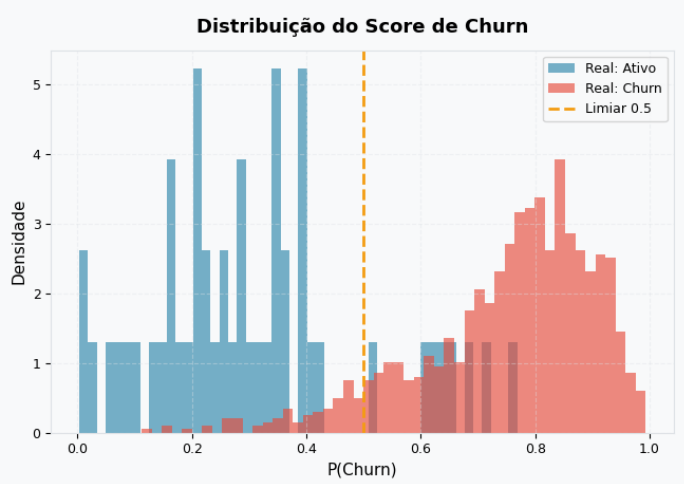
\includegraphics[width=0.9\textwidth]{USPSC-img/figuras/fig03-eda-recencia.png}
\end{center}
\begin{flushleft}
	\ABNTEXfontereduzida
	\SingleSpacing
	Fonte: elaborado pelo autor.
\end{flushleft}
\end{figure}

\begin{figure}[htbp]
\caption{Análise exploratória de frequência}
\label{fig:eda-frequencia}
\begin{center}
	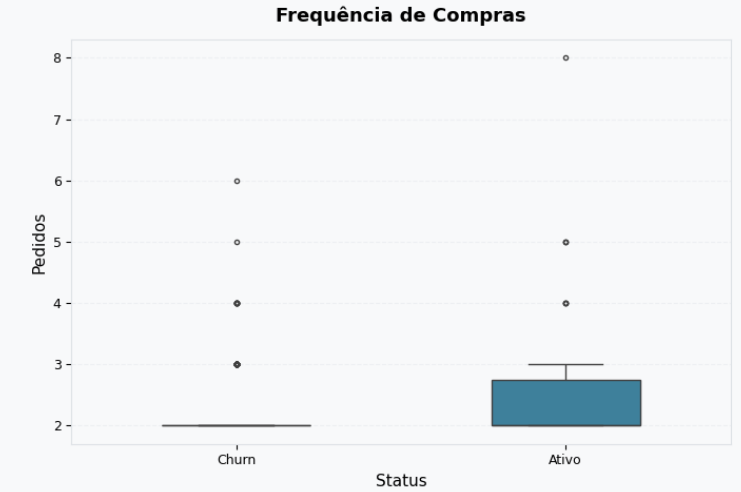
\includegraphics[width=0.9\textwidth]{USPSC-img/figuras/fig04-eda-frequencia.png}
\end{center}
\begin{flushleft}
	\ABNTEXfontereduzida
	\SingleSpacing
	Fonte: elaborado pelo autor.
\end{flushleft}
\end{figure}

\begin{figure}[htbp]
\caption{Análise exploratória de review score}
\label{fig:eda-review}
\begin{center}
	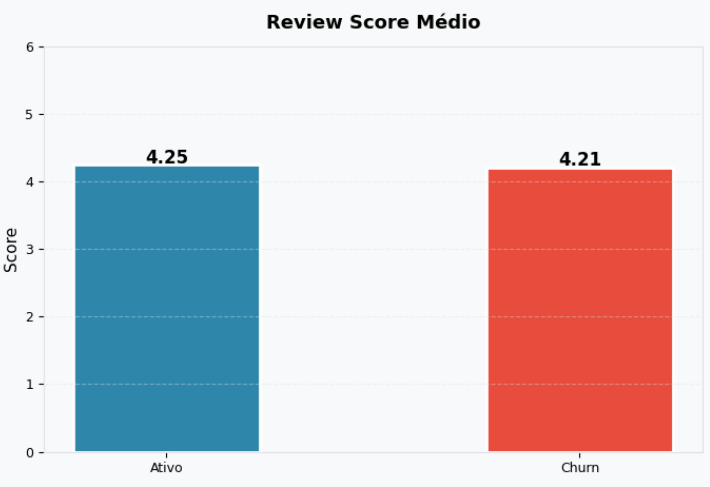
\includegraphics[width=0.9\textwidth]{USPSC-img/figuras/fig05-eda-review-score.png}
\end{center}
\begin{flushleft}
	\ABNTEXfontereduzida
	\SingleSpacing
	Fonte: elaborado pelo autor.
\end{flushleft}
\end{figure}

\begin{figure}[htbp]
\caption{Proporção Churn versus Ativo}
\label{fig:proporcao-classes}
\begin{center}
	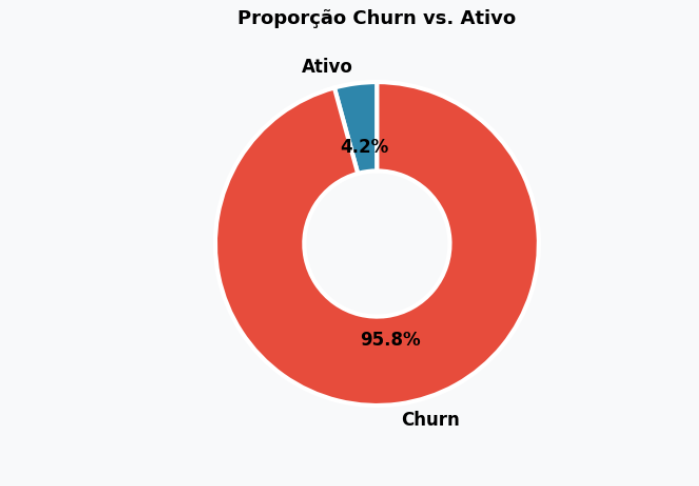
\includegraphics[width=0.7\textwidth]{USPSC-img/figuras/fig06-proporcao-churn-ativo.png}
\end{center}
\begin{flushleft}
	\ABNTEXfontereduzida
	\SingleSpacing
	Fonte: elaborado pelo autor.
\end{flushleft}
\end{figure}

\FloatBarrier
\section{Benchmark Comparativo de Algoritmos} \label{sec:benchmark}

A Tabela \ref{tab:benchmark} apresenta os resultados consolidados dos dez algoritmos avaliados, ordenados por ROC-AUC no conjunto de teste e acompanhados das métricas complementares MCC, G-Mean e Kappa, cujos rankings são analisados na Seção \ref{sec:correlacao-rankings}. O Random Forest obteve o melhor desempenho em termos de discriminação global (AUC = 0,8106), seguido pelo HistGradient Boosting (AUC = 0,7615) e pelo Extra Trees (AUC = 0,7491). No extremo oposto, a Árvore de Decisão apresentou o pior resultado (AUC = 0,4772), valor inferior ao do classificador aleatório, cujo AUC teórico é 0,50 \cite{fawcett2006}, seguida pelo KNN (AUC = 0,5336). Em ambos os casos, o desempenho aproxima-se ou situa-se abaixo do classificador aleatório, resultado discutido adiante à luz do protocolo de validação adotado.

\begin{table}[htbp]
\ABNTEXfontereduzida
\SingleSpacing
\caption{Benchmark comparativo dos dez algoritmos de Machine Learning}
\label{tab:benchmark}
\centering
\scriptsize
\setlength{\tabcolsep}{2.2pt}
\begin{tabular}{@{}>{\raggedright\arraybackslash}p{2.3cm}rrrrrrrrrrrr@{}}
\hline
\textbf{Modelo} & \textbf{AUC} & \textbf{AP} & \shortstack[r]{\textbf{CV-}\\\textbf{AUC}} & \textbf{$\Delta$} & \shortstack[r]{\textbf{F1-}\\\textbf{Macro}} & \textbf{MCC} & \shortstack[r]{\textbf{G-}\\\textbf{Mean}} & \textbf{Kappa} & \shortstack[r]{\textbf{Prec.}\\\textbf{Ativo}} & \shortstack[r]{\textbf{Rec.}\\\textbf{Ativo}} & \shortstack[r]{\textbf{Rec.}\\\textbf{Churn}} & \textbf{Limiar} \\
\hline
Random Forest & 0,8106 & 0,9905 & 0,6814 & 0,1293 & 0,5957 & 0,1931 & 0,4412 & 0,1918 & 0,2500 & 0,20 & 0,9735 & 0,38 \\
HistGradient Boosting & 0,7615 & 0,9872 & 0,7363 & 0,0252 & 0,6049 & 0,2143 & 0,5342 & 0,2110 & 0,2143 & 0,30 & 0,9513 & 0,18 \\
Extra Trees & 0,7491 & 0,9860 & 0,6777 & 0,0714 & 0,5649 & 0,1639 & 0,3148 & 0,1370 & 0,3333 & 0,10 & 0,9912 & 0,34 \\
Regressão Logística & 0,7075 & 0,9838 & 0,6326 & 0,0749 & 0,6440 & 0,3517 & 0,4462 & 0,2939 & 0,6667 & 0,20 & 0,9956 & 0,12 \\
SVM & 0,7035 & 0,9833 & 0,6238 & 0,0798 & 0,4920 & 0,0250 & 0,4111 & 0,0197 & 0,0541 & 0,20 & 0,8451 & 0,37 \\
Gradient Boosting & 0,6642 & 0,9796 & 0,6695 & 0,0053 & 0,5339 & 0,0679 & 0,3106 & 0,0678 & 0,1111 & 0,10 & 0,9646 & 0,08 \\
Naive Bayes & 0,6405 & 0,9552 & 0,6390 & 0,0015 & 0,5887 & 0,1778 & 0,4402 & 0,1775 & 0,2222 & 0,20 & 0,9690 & 0,01 \\
AdaBoost & 0,5544 & 0,9694 & 0,5372 & 0,0172 & 0,5725 & 0,2100 & 0,3155 & 0,1547 & 0,5000 & 0,10 & 0,9956 & 0,47 \\
KNN & 0,5336 & 0,9596 & 0,5913 & 0,0577 & 0,5143 & 0,0314 & 0,3063 & 0,0307 & 0,0667 & 0,10 & 0,9381 & 0,09 \\
Árvore de Decisão & 0,4772 & 0,9559 & 0,6119 & 0,1347 & 0,4592 & 0,0178 & 0,4708 & 0,0112 & 0,0484 & 0,30 & 0,7389 & 0,61 \\
\hline
\end{tabular}
\begin{flushleft}
	\ABNTEXfontereduzida
	\SingleSpacing
	Fonte: elaborado pelo autor.

	\textit{Nota: $\Delta$ é a diferença absoluta entre CV-AUC e AUC no hold-out. AP designa a Average Precision para a classe Churn, cuja linha de base no conjunto de teste é 0,958, valor correspondente à prevalência dessa classe; a informação relevante nessa coluna é a comparação entre modelos, e não a magnitude absoluta. Rec. Ativo corresponde à proporção das dez instâncias da classe Ativo do conjunto de teste corretamente identificadas. O limiar de cada modelo foi derivado das probabilidades out-of-fold do conjunto de treino, conforme a Seção \ref{sec:protocolo}, e todas as métricas dependentes de limiar foram calculadas nesse valor. Nenhum modelo foi descartado pelo critério de diferença entre validação cruzada e hold-out.}
\end{flushleft}
\end{table}

A validação cruzada, conduzida com a reamostragem aplicada dentro de cada partição, não indicou sobreajuste em nenhum dos dez algoritmos: a maior diferença em relação ao hold-out foi de 0,1347 (Árvore de Decisão), seguida de 0,1293 (Random Forest), ambas abaixo do limite de 0,15 fixado na Seção \ref{sec:protocolo}. Registra-se a sensibilidade a esse parâmetro: sob um corte de 0,10, esses dois algoritmos seriam descartados, entre eles o adotado como modelo de produção; sob 0,20, o resultado seria idêntico ao obtido. Como nenhum modelo foi excluído pelo critério, ele não participou da escolha do modelo de produção, que se apoia nos fundamentos expostos adiante nesta seção. Esse resultado contrasta com o obtido na concepção inicial deste trabalho, em que a validação cruzada era conduzida sobre o conjunto de treino já balanceado. Naquele protocolo, instâncias sintéticas geradas por perturbação de uma mesma observação original distribuíam-se entre folds distintos, e o modelo avaliava, na partição de validação, quase duplicatas de exemplos vistos no ajuste. O efeito da correção é sistemático e ordena-se pela capacidade de memorização de cada algoritmo: a estimativa de validação cruzada caiu 0,3251 no AdaBoost, 0,3222 no KNN e 0,2657 no Extra Trees, contra apenas 0,0789 na Regressão Logística e 0,0634 no Naive Bayes, modelos paramétricos cuja estrutura não permite memorizar instâncias próximas. O caso do KNN é ilustrativo: sua estimativa de validação cruzada passou de 0,9135 para 0,5913, valor compatível com o desempenho de 0,5336 obtido no hold-out. Conclui-se que a diferença entre validação cruzada e hold-out observada na concepção inicial media vazamento de informação entre partições, e não sobreajuste ao conjunto de treino.

Sob as três métricas recomendadas por De la Cruz Huayanay, Bazán e Russo (\citeyear{delacruz2025}), o modelo indicado seria o HistGradient Boosting: ele lidera o G-Mean (0,5342, o maior valor do conjunto) e ocupa a segunda posição em MCC (0,2143) e em Kappa de Cohen (0,2110). É também um dos dois algoritmos que identificam o maior número de clientes Ativos, três das dez instâncias do hold-out, empatado com a Árvore de Decisão mas com precisão muito superior (0,2143 contra 0,0484), e o que apresenta a menor diferença entre validação cruzada e hold-out entre os três modelos de melhor desempenho (0,0252), além da maior CV-AUC do conjunto (0,7363). A liderança isolada em MCC (0,3517) e Kappa (0,2939) cabe, contudo, à Regressão Logística, cuja vantagem não se sustenta na classe minoritária: o modelo identifica as mesmas duas instâncias Ativas que o Random Forest, e sua superioridade decorre integralmente da redução de falsos negativos, isto é, de clientes Churn incorretamente classificados como Ativos (um caso contra seis). Trata-se do mesmo padrão registrado na Seção \ref{sec:target-balanceamento} a respeito da ausência de balanceamento. O Random Forest, por sua vez, lidera a ROC-AUC (0,8106) e a Average Precision para a classe Churn (0,9905), as duas métricas do conjunto que independem do limiar de classificação e que medem, portanto, a qualidade da ordenação dos clientes por risco.

Os valores absolutos de MCC e Kappa de Cohen, com máximos de 0,35 e 0,29 respectivamente entre os dez modelos, situam-se abaixo do limiar usualmente associado a concordância substancial \cite{landis1977}. É importante enfatizar que essa limitação decorre estruturalmente da composição do conjunto de teste: com apenas dez instâncias da classe Ativo em um hold-out de 236 clientes, no qual a proporção de 4,2\% da base foi preservada, qualquer erro de classificação na classe minoritária impacta desproporcionalmente o MCC e o Kappa, comportamento previsto analiticamente por \citeonline{luque2019} e coerente com a sensibilidade do MCC a todos os quadrantes da matriz de confusão, destacada por \citeonline{chicco2020}. A mesma escassez restringe o número de configurações possíveis da matriz de confusão: o Recall da classe Ativo assume apenas três valores distintos entre os dez algoritmos avaliados (0,10, 0,20 e 0,30), e nenhum modelo ultrapassa três acertos em dez. Não se trata de falha algorítmica, mas de consequência matemática do desbalanceamento extremo preservado no hold-out, escolha metodológica deliberada para preservar a validade da avaliação em condições reais de operação.

Os três modelos de melhor desempenho, Random Forest, HistGradient Boosting e Regressão Logística, apresentam perfis distintos de vantagens e desvantagens, sintetizados no Quadro \ref{qua:tres-modelos}. A inclusão da Regressão Logística no quadro decorre de sua liderança isolada em MCC e Kappa de Cohen: sob as métricas recomendadas por De la Cruz Huayanay, Bazán e Russo (\citeyear{delacruz2025}), ela é candidata obrigatória, ainda que a literatura a trate como modelo de referência e não como concorrente dos ensembles \cite{prabadevi2023}. A escolha entre os três não é absoluta, mas está condicionada ao objetivo do negócio e à estrutura de custos da operação de retenção.

\begingroup
% Reserva espaco para que a legenda nao fique separada da primeira linha do quadro
\Needspace*{10\baselineskip}
\quadrocaption{Análise de vantagens e desvantagens dos três modelos de melhor desempenho}
\label{qua:tres-modelos}
\ABNTEXfontereduzida
\SingleSpacing
\begin{longtable}{|>{\raggedright\arraybackslash}p{2.3cm}|>{\raggedright\arraybackslash}p{5.6cm}|>{\raggedright\arraybackslash}p{5.6cm}|}
\hline
\textbf{Modelo} & \textbf{Vantagens} & \textbf{Desvantagens} \\
\hline
\endfirsthead
\hline
\textbf{Modelo} & \textbf{Vantagens} & \textbf{Desvantagens} \\
\hline
\endhead
\hline
\endfoot
\hline
\endlastfoot
Random Forest (produção) &
Maior ROC-AUC (0,8106) e maior Average Precision para a classe Churn (0,9905), as duas métricas que independem do limiar e medem a qualidade da ordenação dos clientes por risco; melhor captura de clientes Ativos em cobertura fixa, liderando ou empatando em todas as frações avaliadas entre 10\% e 60\% do conjunto de teste; alcança 90\% dos clientes Ativos abordando 35,6\% das observações, a menor cobertura entre os três modelos; retém nove dos dez clientes Ativos do conjunto de teste fora da faixa Crítico, em 39,0\% das observações, lift de 2,31 vezes; importância de features nativa via impureza de Gini, requisito do objetivo específico (\ref{obj:importancia}). &
Menores MCC (0,1931), Kappa de Cohen (0,1918) e G-Mean (0,4412) entre os três modelos; identifica duas das dez instâncias Ativas do hold-out, contra três do HistGradient Boosting; menor Average Precision para a classe Ativo (0,1494, contra 0,2559 do HistGradient Boosting), métrica dominada pelo extremo inicial da ordenação; maior diferença entre validação cruzada e hold-out entre os três (0,1293); ROC-AUC média em validação cruzada de 0,6814, inferior aos 0,7363 do HistGradient Boosting; maior custo de memória em produção. \\
\hline
HistGradient Boosting (alternativo) &
Lidera o G-Mean (0,5342, o maior valor do conjunto de dez algoritmos); segundo maior MCC (0,2143) e Kappa de Cohen (0,2110); identifica três das dez instâncias Ativas do hold-out, o maior número entre os três modelos; maior Average Precision para a classe Ativo entre os três (0,2559), o que indica acerto no extremo inicial da ordenação; maior CV-AUC do conjunto (0,7363) e menor diferença em relação ao hold-out entre os três (0,0252); treino rápido em dados tabulares. &
ROC-AUC de 0,7615, inferior aos 0,8106 do Random Forest; scores concentrados no extremo superior da escala (primeiro quartil de 0,7927 e mediana de 0,9621, contra 0,6545 e 0,7781 do Random Forest), o que aloca 77,6\% da base completa e 79,7\% do conjunto de teste na faixa Crítico, reduzindo as demais faixas a 9,6\%, 5,6\% e 7,2\% na base completa e a 8,1\%, 5,9\% e 6,4\% no conjunto de teste; captura menos clientes Ativos que o Random Forest em todas as coberturas entre 20\% e 50\% do conjunto de teste, e requer 49,6\% de cobertura para alcançar 90\% dos Ativos, contra 35,6\% do Random Forest; retém três dos dez clientes Ativos fora da faixa Crítico, em 20,3\% das observações, lift de 1,48 vezes; menor Recall da classe Churn entre os três (0,9513); o HistGradientBoostingClassifier não expõe medida nativa de importância de features, o que inviabiliza a análise de estabilidade da ordenação por Gini conduzida na Seção \ref{sec:interpretabilidade}. \\
\hline
Regressão Logística (referência sob métricas de decisão binária) &
Lidera isoladamente o MCC (0,3517) e o Kappa de Cohen (0,2939), duas das três métricas recomendadas por De la Cruz Huayanay, Bazán e Russo (\citeyear{delacruz2025}); maior Precisão na classe Ativo (0,6667) e maior Recall na classe Churn (0,9956) entre os dez algoritmos; distribuição de scores mais dispersa dos três modelos (intervalo interquartílico de 0,3614, contra 0,2056 do Random Forest), ocupando as quatro faixas de risco de forma mais uniforme (5,8\%, 31,2\%, 33,4\% e 29,6\% na base completa); modelo paramétrico, de baixo custo computacional e interpretação direta por coeficientes, cuja estrutura não permite memorizar instâncias, o que se reflete na queda de apenas 0,0789 entre a estimativa de validação cruzada vazada e a corrigida. &
Menor ROC-AUC entre os três (0,7075) e menor Average Precision para a classe Churn (0,9838); pior captura de clientes Ativos em cobertura fixa, com dois dos dez em 20\% do conjunto de teste, contra quatro do Random Forest, e lift de 0,98 vezes nessa cobertura, valor indistinguível do acaso; requer 52,5\% de cobertura para alcançar 90\% dos clientes Ativos, a maior dos três modelos, e 66,9\% das observações para reter dez dos dez Ativos fora da faixa Crítico, lift de 1,49 vezes; sua vantagem em MCC e Kappa decorre integralmente da redução de falsos negativos na classe majoritária (um caso contra seis do Random Forest) e não de ganho na classe Ativo, na qual identifica as mesmas duas instâncias; não dispõe de medida de importância por impureza, requisito do objetivo específico (\ref{obj:importancia}). \\
\end{longtable}
\begin{flushleft}
	\ABNTEXfontereduzida
	\SingleSpacing
	Fonte: elaborado pelo autor.
\end{flushleft}
\addtocounter{table}{-1}
\endgroup

A seleção do modelo de produção seguiu dois critérios, ordenados pela natureza do entregável descrito na Seção \ref{sec:segmentacao}. O primeiro é a qualidade da ordenação dos clientes por risco. A estratificação em faixas não constitui uma decisão binária em um ponto de corte, mas uma priorização que depende da posição relativa de cada cliente na escala de scores; as métricas apropriadas a esse uso são, portanto, aquelas que independem do limiar, e o Random Forest lidera ambas (ROC-AUC de 0,8106 e Average Precision de 0,9905 para a classe Churn). Cabe registrar que a Average Precision da classe Churn parte de uma linha de base de 0,958, de modo que sua magnitude absoluta é pouco informativa e apenas a ordenação entre modelos o é. A evidência decisiva da qualidade da ordenação não é, por isso, nenhuma das duas métricas isoladamente, mas a curva de captura em cobertura fixa apresentada adiante nesta seção, que independe de linha de base e mede diretamente quantos clientes recuperáveis cada modelo entrega por unidade de esforço. Cabe explicitar que a vantagem do Random Forest reside na ordenação dos clientes, e não na dispersão de seus scores. A Figura \ref{fig:distribuicao-scores} evidencia que a Regressão Logística produz a distribuição mais uniforme entre as quatro faixas (5,8\%, 31,2\%, 33,4\% e 29,6\% na base completa, contra 2,3\%, 8,6\%, 31,0\% e 58,1\% do Random Forest), e ainda assim é a menos eficaz na identificação de clientes recuperáveis por unidade de cobertura. O segundo critério é, portanto, a eficiência do recorte resultante, verificada empiricamente no conjunto de teste e detalhada nos parágrafos seguintes. Registra-se explicitamente que, sob as três métricas recomendadas por De la Cruz Huayanay, Bazán e Russo (\citeyear{delacruz2025}), aplicáveis à avaliação de decisões binárias, o modelo de produção não seria o Random Forest, que ocupa a quarta posição em MCC e em G-Mean e a terceira em Kappa de Cohen. A escolha recairia sobre o HistGradient Boosting ou sobre a Regressão Logística, que empatam em posição média nos três rankings (1,67 cada), o primeiro por liderar o G-Mean e a segunda por liderar MCC e Kappa. Esse empate é ilustrativo: as métricas recomendadas apontam a inadequação do Random Forest para a decisão binária, mas não desempatam entre si, o que reforça que o critério de escolha precisa vir da natureza do entregável. A divergência entre os dois conjuntos de critérios não é resolvida por arbitragem entre métricas, mas pela definição do que o modelo entrega: adota-se o Random Forest porque o produto deste trabalho é uma priorização de risco, e o HistGradient Boosting permanece registrado como alternativa indicada caso o objetivo passe a ser a maximização da detecção da classe minoritária em regime de decisão binária.

Registra-se, ademais, uma limitação operacional do HistGradient Boosting relativa à distribuição de suas probabilidades preditas. Aplicado à base completa, esse modelo concentra os scores junto do extremo superior da escala (primeiro quartil de 0,7927, mediana de 0,9621 e terceiro quartil de 0,9915), enquanto o Random Forest mantém a distribuição centrada em valores intermediários da escala (primeiro quartil de 0,6545, mediana de 0,7781 e terceiro quartil de 0,8601) e a Regressão Logística, a mais dispersa das três (primeiro quartil de 0,4204, mediana de 0,6000 e terceiro quartil de 0,7818). Esse deslocamento das probabilidades para a classe majoritária do treino é coerente com o viés induzido pelo treinamento em conjunto artificialmente balanceado, formalizado por \citeonline{dalpozzolo2015}, e manifesta-se de forma mais acentuada no HistGradient Boosting do que nos demais, sem prejuízo da ordenação relativa dos clientes, o que explica a preservação de seu ROC-AUC. A consequência prática recai sobre a granularidade da segmentação de risco em faixas apresentada na Seção \ref{sec:segmentacao}. Aplicados os mesmos limiares da Tabela \ref{tab:segmentacao} à base completa, o HistGradient Boosting aloca 77,6\% dos clientes na faixa Crítico e distribui os demais em 9,6\% no Baixo, 5,6\% no Médio e 7,2\% no Alto, contra 58,1\%, 2,3\%, 8,6\% e 31,0\% do Random Forest e 29,6\%, 5,8\%, 31,2\% e 33,4\% da Regressão Logística, respectivamente. O mesmo padrão reproduz-se no conjunto de teste, o que afasta a hipótese de artefato das observações de treino: nele o HistGradient Boosting aloca 79,7\% dos clientes na faixa Crítico, restando 8,1\% no Baixo, 5,9\% no Médio e 6,4\% no Alto, enquanto o Random Forest aloca 61,0\% no Crítico, 30,9\% no Alto, 6,4\% no Médio e 1,7\% no Baixo, e a Regressão Logística, 33,1\%, 31,8\%, 30,1\% e 5,1\%. A escala do modelo alternativo comporta, portanto, essencialmente uma faixa útil, o que compromete a capacidade de priorizar clientes por grau de risco. Registra-se, contudo, que a dispersão da escala não é, isoladamente, critério de escolha: a Regressão Logística apresenta a distribuição mais uniforme dos três modelos e o pior desempenho na identificação de clientes recuperáveis por unidade de cobertura, conforme se demonstra a seguir.

Cabe dimensionar o trade-off em termos absolutos. A vantagem do HistGradient Boosting na detecção da classe minoritária corresponde a um cliente Ativo adicional identificado entre os dez do conjunto de teste, ao custo de onze falsos negativos na classe Churn contra seis do Random Forest. Do ponto de vista da operação de retenção, a comparação relevante é a concentração de clientes Ativos nas faixas de menor risco, necessariamente restrita ao conjunto de teste, uma vez que a base completa contém as observações utilizadas no ajuste. Nesse recorte, o Random Forest reúne dois dos dez clientes Ativos em 8,1\% das observações, lift de 2,48 vezes, e o HistGradient Boosting reúne três em 14,0\%, lift de 2,15 vezes. A diferença entre os dois valores corresponde a um único cliente e não autoriza afirmar superioridade de qualquer dos modelos, de modo que esse critério não se presta ao desempate. Adotando-se o recorte complementar, a exclusão da faixa Crítico, o Random Forest retém nove dos dez clientes Ativos em 39,0\% do conjunto de teste, lift de 2,31 vezes, contra três dos dez em 20,3\% do HistGradient Boosting, lift de 1,48 vezes, e dez dos dez em 66,9\% da Regressão Logística, lift de 1,49 vezes. A Regressão Logística alcança a totalidade dos clientes Ativos, mas ao custo de abordar dois terços do conjunto de teste, cobertura que descaracteriza o próprio propósito da priorização.

Os três recortes acima entregam frações distintas do conjunto de teste, o que faz o lift refletir simultaneamente a qualidade da ordenação e o ponto em que o corte de 75\% incide sobre a distribuição de cada modelo. Para isolar a ordenação, os clientes foram ordenados do menor para o maior score e mediu-se, em coberturas fixas, quantos dos dez clientes Ativos do conjunto de teste seriam alcançados. O Random Forest lidera ou empata em todas as coberturas avaliadas: em 30\% das observações captura oito dos dez clientes Ativos, contra seis do HistGradient Boosting e cinco da Regressão Logística; em 40\%, nove contra oito e sete; e em 50\%, dez contra nove e oito. Consequentemente, alcança 90\% dos clientes Ativos abordando 35,6\% do conjunto de teste, contra 49,6\% do HistGradient Boosting e 52,5\% da Regressão Logística. Abaixo de 30\% de cobertura nenhum dos três modelos ultrapassa quatro acertos em dez, e a partir de 60\% os três alcançam a totalidade dos Ativos, de modo que a escolha do modelo só produz efeito operacional relevante no intervalo intermediário, precisamente aquele em que o Random Forest apresenta vantagem. Cabe a ressalva de que o conjunto de teste contém apenas dez clientes Ativos, de modo que cada unidade capturada equivale a dez pontos percentuais de Recall e diferenças de um único cliente não são conclusivas.

Some-se a isso que o HistGradientBoostingClassifier não expõe medida nativa de importância de features. A análise de interpretabilidade conduzida na Seção \ref{sec:interpretabilidade}, requisito do objetivo específico (\ref{obj:importancia}), apoia-se na importância por impureza de Gini e na estabilidade dessa ordenação em trinta partições estratificadas, ambas indisponíveis para o modelo alternativo. Os valores SHAP permaneceriam calculáveis, e são efetivamente empregados na Tabela \ref{tab:shap-tres-modelos} como terreno comum de comparação entre os três modelos, mas isoladamente não reproduziriam a evidência de estabilidade, que é estimada sobre a ordenação por Gini. Replicar a análise exigiria substituir o estimador pela importância por permutação, que a própria Seção \ref{sec:interpretabilidade} mostra não ser informativa neste regime amostral, ajuste que extrapola o escopo deste trabalho. O HistGradient Boosting permanece recomendado como alternativa, condicionada à aplicação prévia de técnicas de calibração de probabilidades, como Platt scaling ou regressão isotônica, cuja eficácia na correção de probabilidades produzidas por boosting foi demonstrada empiricamente por \citeonline{niculescu2005}, especialmente em contextos de custo por contato elevado, nos quais a redução de falsos positivos é prioritária.

\FloatBarrier
\section{Correlação entre Rankings de Métricas} \label{sec:correlacao-rankings}

A análise de correlação de Spearman entre os rankings dos dez modelos revelou comportamento heterogêneo entre as métricas avaliadas. Os rankings por ROC-AUC e por Kappa de Cohen apresentam a correlação mais elevada do conjunto (rho = 0,6485), única estatisticamente significativa ao nível de 5\% (p = 0,043). A correlação com o ranking por MCC é moderada e não significativa (rho = 0,5515; p = 0,098), e a correlação com o ranking por G-Mean é fraca (rho = 0,2970; p = 0,405), indicando que essas duas métricas ordenam os modelos de maneira substancialmente distinta.

A divergência é evidenciada de forma direta pelo próprio ranking, que produz três vencedores distintos entre os quatro critérios avaliados: o Random Forest lidera a ROC-AUC (0,8106), o HistGradient Boosting lidera o G-Mean (0,5342) e a Regressão Logística lidera simultaneamente o MCC (0,3517) e o Kappa (0,2939). Nenhum dos três modelos ocupa a primeira posição em mais de dois dos quatro critérios, e o líder por ROC-AUC figura apenas na quarta posição do ranking de G-Mean.

Esse resultado converge com a recomendação de De la Cruz Huayanay, Bazán e Russo (\citeyear{delacruz2025}) contra o uso isolado da ROC-AUC, ainda que por evidência de natureza distinta: enquanto aqueles autores avaliam, em simulação, a capacidade de cada métrica de identificar o modelo verdadeiro, este trabalho observa a divergência entre rankings de modelos em dados reais. A fraca associação entre os rankings de ROC-AUC e G-Mean justifica a adoção do portfólio de métricas complementares utilizado neste trabalho e reforça a necessidade de que estudos comparativos de churn em e-commerce não se limitem à ROC-AUC como único critério avaliativo. Cabe registrar, contudo, que os coeficientes foram estimados sobre apenas dez observações, de modo que os valores devem ser interpretados como indicativos da tendência observada neste conjunto de modelos, e não como estimativas populacionais precisas; apenas uma das três correlações atinge significância ao nível de 5\%.

\FloatBarrier
\section{Análise do Limiar de Classificação e Curvas de Desempenho} \label{sec:limiar}

A análise do ponto de corte para o Random Forest, apresentada na Figura \ref{fig:limiar-corte}, indicou que o limiar que maximiza o Kappa de Cohen sobre as probabilidades out-of-fold do conjunto de treino situa-se em 0,38, abaixo do valor padrão de 0,50 \cite{fawcett2006}. Esse resultado decorre do treinamento em um conjunto balanceado artificialmente, procedimento que altera as probabilidades a priori e, por consequência, enviesa as probabilidades posteriores estimadas pelo modelo, fenômeno formalizado analiticamente por \citeonline{dalpozzolo2015}. O deslocamento é evidenciado pela própria distribuição das probabilidades preditas no conjunto de teste, cuja mediana é de 0,779 e cujo valor mínimo é de 0,112, indicando concentração na faixa superior da escala. A proximidade entre as distribuições out-of-fold do treino (mediana de 0,772) e do hold-out (mediana de 0,779) confirma que o limiar derivado da primeira transfere-se adequadamente ao segundo.

Cabe dimensionar o efeito do procedimento de derivação do limiar. O valor de 0,38, obtido sobre o conjunto de treino, produz Kappa de 0,1918 no hold-out. Caso o limiar fosse selecionado diretamente sobre o conjunto de teste, como na concepção inicial deste trabalho, o valor escolhido seria 0,34 e o Kappa reportado seria 0,2254. A diferença de 0,0336 entre os dois valores corresponde exatamente ao viés otimista que a seleção do limiar no conjunto de avaliação incorpora ao resultado, e a magnitude desse viés não pode ser conhecida sem que se disponha do procedimento correto como referência. Todas as métricas dependentes de limiar reportadas neste trabalho foram calculadas no limiar derivado do treino.

No limiar padrão de 0,50, 91,9\% dos clientes de teste são classificados como Churn, proporção inferior à real (95,8\%), o que indica que parte dos clientes que de fato não retornaram recebe probabilidade prevista abaixo de 0,50 e seria incorretamente classificada como Ativo. A redução do limiar para 0,38 atenua esse deslocamento, ampliando a cobertura da classe majoritária ao custo de maior número de falsos positivos, isto é, de clientes Ativos incorretamente classificados como Churn, trade-off dimensionado na Seção \ref{sec:benchmark}. Cabe registrar que o viés decorrente do balanceamento afeta as métricas dependentes de limiar, mas não a ordenação das probabilidades preditas \cite{dalpozzolo2015}, o que corrobora a adoção de métricas independentes de limiar como critério primário de seleção.

As matrizes de confusão resultantes (Figuras \ref{fig:matrizes-a} e \ref{fig:matrizes-b}) confirmam a elevada capacidade de identificação da classe Churn, com Recall de 0,97 (220 das 226 instâncias), e evidenciam, ao mesmo tempo, a limitação imposta pela classe Ativo, representada por apenas dez instâncias no conjunto de teste, das quais duas são corretamente identificadas. O teto observado entre os dez algoritmos avaliados é de três acertos em dez (Tabela \ref{tab:benchmark}), obtido pelo HistGradient Boosting e pela Árvore de Decisão, o que situa o desempenho do modelo de produção próximo ao máximo alcançável neste regime amostral e reforça que a limitação é da base, e não do algoritmo.

\begin{figure}[htbp]
\caption{Matrizes de confusão do Logistic Regression, Decision Tree, HistGradient Boosting, AdaBoost e KNN no conjunto de teste (limiar out-of-fold)}
\label{fig:matrizes-a}
\begin{center}
	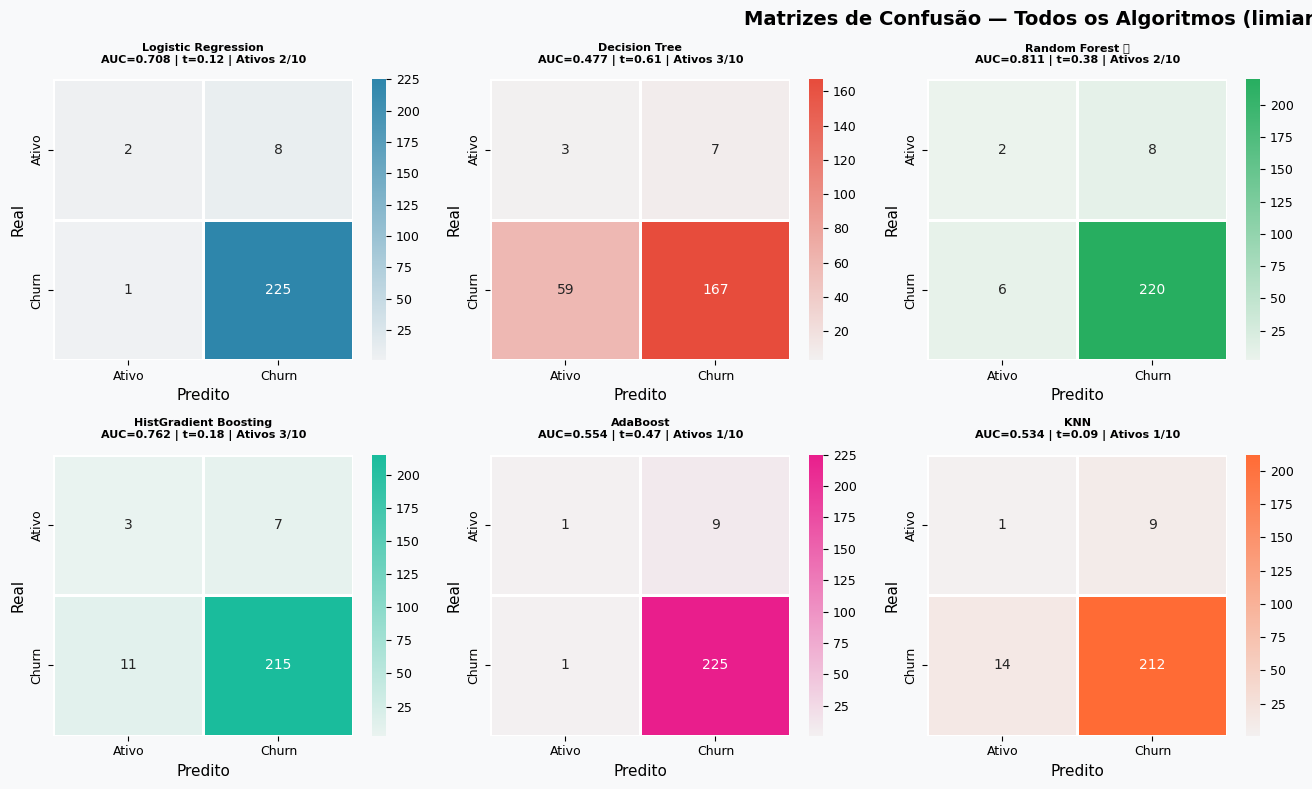
\includegraphics[width=0.95\textwidth]{USPSC-img/figuras/fig07-matrizes-confusao-a.png}
\end{center}
\begin{flushleft}
	\ABNTEXfontereduzida
	\SingleSpacing
	Fonte: elaborado pelo autor.
\end{flushleft}
\end{figure}

\begin{figure}[htbp]
\caption{Matrizes de confusão do Extra Trees, Gradient Boosting, Naive Bayes e SVM no conjunto de teste (limiar out-of-fold)}
\label{fig:matrizes-b}
\begin{center}
	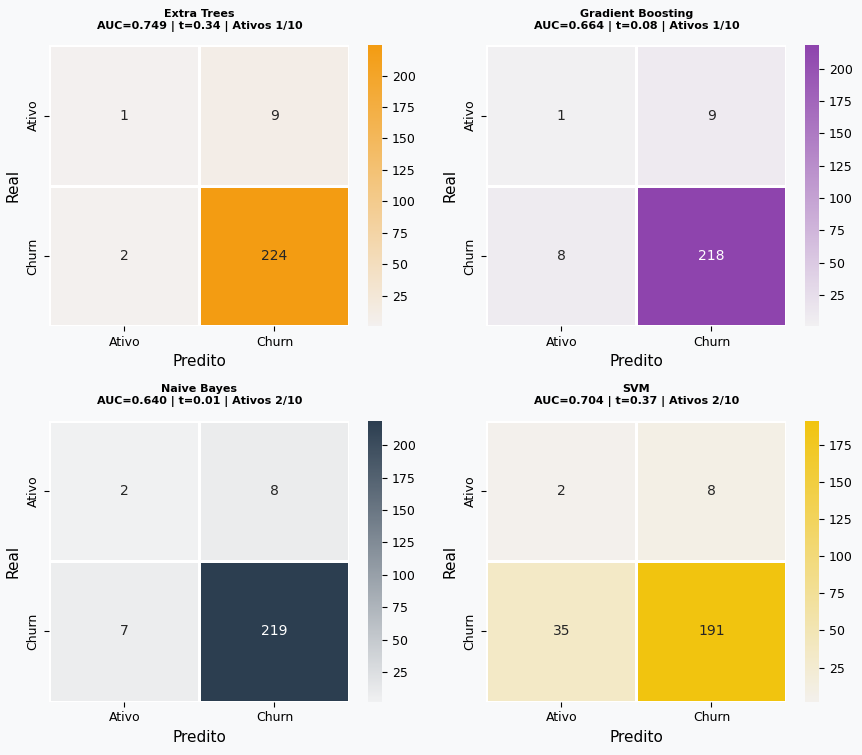
\includegraphics[width=0.95\textwidth]{USPSC-img/figuras/fig08-matrizes-confusao-b.png}
\end{center}
\begin{flushleft}
	\ABNTEXfontereduzida
	\SingleSpacing
	Fonte: elaborado pelo autor.
\end{flushleft}
\end{figure}

A Curva Precision-Recall (Figura \ref{fig:curva-pr}) corrobora a qualidade preditiva do modelo, análise especialmente apropriada em desbalanceamento severo \cite{saito2015}. A Average Precision (AP) para a classe Churn é de 0,9905, valor que deve ser lido contra a linha de base de 0,958 correspondente à prevalência dessa classe no conjunto de teste. A informação útil dessa métrica está, portanto, na comparação entre modelos, e não em sua magnitude absoluta, que é estruturalmente alta em qualquer classificador sob esse grau de desbalanceamento. Para a classe Ativo, minoritária, a AP situa-se em 0,1494, aproximadamente 3,5 vezes o baseline de um classificador aleatório (0,042), desempenho superior ao acaso, mas limitado pela escassez de exemplos positivos, apenas dez instâncias no conjunto de teste. Os valores correspondentes nos dois modelos concorrentes são de 0,2559 no HistGradient Boosting e 0,1749 na Regressão Logística, divergência analisada na Seção \ref{sec:benchmark}.

\begin{figure}[htbp]
\caption{Critério de escolha do ponto de corte em função do limiar (Random Forest)}
\label{fig:limiar-corte}
\begin{center}
	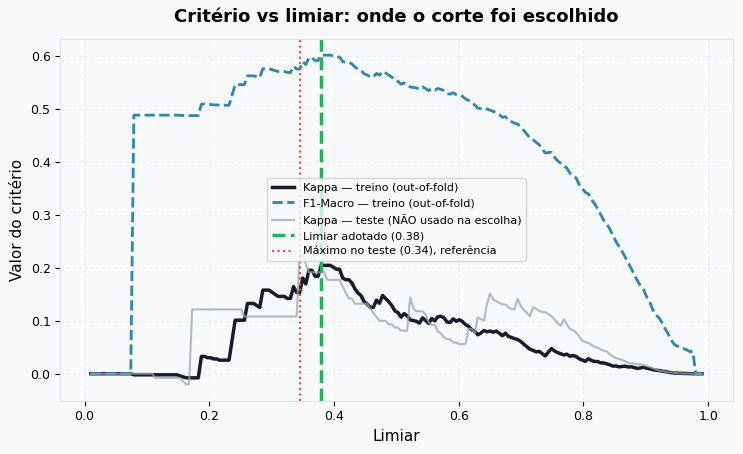
\includegraphics[width=0.9\textwidth]{USPSC-img/figuras/fig09-limiar-corte.png}
\end{center}
\begin{flushleft}
	\ABNTEXfontereduzida
	\SingleSpacing
	Fonte: elaborado pelo autor.
\end{flushleft}
\end{figure}

\begin{figure}[htbp]
\caption{Curva Precision-Recall por classe, independente do limiar (Random Forest)}
\label{fig:curva-pr}
\begin{center}
	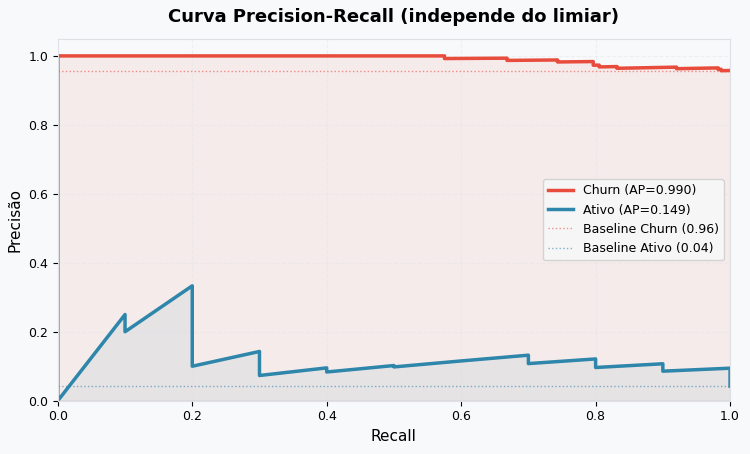
\includegraphics[width=0.9\textwidth]{USPSC-img/figuras/fig10-curva-precision-recall.png}
\end{center}
\begin{flushleft}
	\ABNTEXfontereduzida
	\SingleSpacing
	Fonte: elaborado pelo autor.
\end{flushleft}
\end{figure}

\FloatBarrier
\section{Validação da Representatividade do Balanceamento} \label{sec:representatividade}

A fim de verificar se o subconjunto da classe Churn retido no treino após o undersampling aleatório preserva a distribuição estatística da classe original \cite{he2009}, foram aplicados dois testes complementares: o Population Stability Index (PSI) e o teste de Kolmogorov-Smirnov (KS). A comparação contrapõe as 1.128 observações da classe Churn completa às 120 efetivamente utilizadas no treino após o undersampling na razão 3:1, correspondentes a uma taxa de retenção de 10,6\%. A Tabela \ref{tab:psi-ks} apresenta os resultados para as nove features numéricas.

\begin{table}[htbp]
\ABNTEXfontereduzida
\SingleSpacing
\caption{Validação de representatividade via PSI e KS-test (features numéricas)}
\label{tab:psi-ks}
\centering
\scriptsize
\setlength{\tabcolsep}{4pt}
\begin{tabular}{@{}lcrrrrrl@{}}
\hline
\textbf{Feature} & \textbf{Tipo} & \shortstack[r]{\textbf{N}\\\textbf{Completo}} & \shortstack[r]{\textbf{N}\\\textbf{Retido}} & \textbf{PSI} & \textbf{KS} & \textbf{p-valor} & \textbf{Status} \\
\hline
recency\_days       & Contínua & 1.128 & 120 & 0,0375 & 0,0574 & 0,845 & Representativa \\
frequency           & Discreta & 1.128 & 120 & 0,0039 & 0,0041 & 1,000 & Representativa \\
monetary            & Contínua & 1.128 & 120 & 0,0209 & 0,0418 & 0,987 & Representativa \\
avg\_ticket         & Contínua & 1.128 & 120 & 0,0265 & 0,0473 & 0,958 & Representativa \\
avg\_delivery\_days & Contínua & 1.128 & 120 & 0,0340 & 0,0537 & 0,896 & Representativa \\
avg\_review\_score  & Contínua & 1.128 & 120 & 0,0103 & 0,0305 & 1,000 & Representativa \\
avg\_installments   & Contínua & 1.128 & 120 & 0,1293 & 0,1035 & 0,182 & Atenção \\
avg\_freight        & Contínua & 1.128 & 120 & 0,0602 & 0,0812 & 0,448 & Representativa \\
n\_categories       & Discreta & 1.128 & 120 & 0,0022 & 0,0101 & 1,000 & Representativa \\
\hline
\end{tabular}
\begin{flushleft}
	\ABNTEXfontereduzida
	\SingleSpacing
	Fonte: elaborado pelo autor.
\end{flushleft}
\end{table}

Oito das nove features apresentaram PSI inferior a 0,10, limiar de instabilidade convencionalmente adotado, com p-valores do teste KS superiores a 0,44, indicando ausência de diferença estatisticamente significativa entre as distribuições. A única exceção é a variável avg\_installments, cujo PSI de 0,1293 situa-se na faixa de atenção, ainda que o teste KS não rejeite a hipótese de igualdade das distribuições (p = 0,182). Nenhuma feature foi classificada como distorcida.

Esses resultados são consistentes com a preservação da distribuição da classe Churn no subconjunto retido. O peso da conclusão recai sobre o PSI: oito das nove features situam-se abaixo de 0,10 e a nona, avg\_installments, permanece na faixa de atenção, sem que nenhuma variável alcance a faixa de distorção. O teste de Kolmogorov-Smirnov entra como verificação complementar, cabendo registrar que a não rejeição da hipótese de igualdade não equivale a demonstrá-la: com 120 observações retidas contra 1.128, a potência do teste é limitada, e diferenças de magnitude moderada não seriam necessariamente detectadas. Tomados em conjunto, os dois indicadores sustentam que o conjunto de treino foi construído sobre uma amostra do Churn real, e não sobre uma versão sistematicamente distorcida da classe majoritária, com desvio restrito a uma única variável de importância intermediária no modelo.

Registra-se que essa verificação alcança o undersampling da classe majoritária. A expansão sintética da classe Ativo, responsável por dois terços das instâncias minoritárias do conjunto de treino, não é objeto do mesmo teste: com quarenta observações originais, os testes empregados teriam potência insuficiente para distinguir a distribuição sintética da original. Sua adequação é discutida qualitativamente no Quadro \ref{qua:estrategias-balanceamento} e na Seção \ref{subsec:clientes-informativos}, e a validação quantitativa da perturbação gaussiana permanece entre os trabalhos futuros.

\subsection{Discussão: representatividade e clientes informativos} \label{subsec:clientes-informativos}

A validação por PSI e KS-test atesta que o undersampling aleatório preserva a distribuição estatística marginal das features. Cabe, contudo, uma reflexão metodológica complementar: a estratégia de seleção aleatória trata todas as observações da classe majoritária como igualmente informativas, hipótese que nem sempre se sustenta. A literatura de aprendizado sensível a instâncias distingue observações seguras, que representam de forma confiável a região central da distribuição, de observações redundantes ou ruidosas, cuja remoção não compromete, e pode até favorecer, a capacidade discriminativa do modelo \cite{kubat1997}.

No contexto deste trabalho, essa perspectiva é particularmente relevante para a classe minoritária, composta por aproximadamente 50 clientes Ativos. Por se tratar de uma amostra reduzida, cada observação da classe Ativo representa parcela expressiva da informação disponível sobre o comportamento de recompra, razão pela qual a perturbação gaussiana adotada no oversampling preserva integralmente as observações originais, em vez de substituí-las por instâncias interpoladas.

Uma extensão natural seria substituir o undersampling aleatório da classe Churn por uma seleção orientada por informatividade, como o one-sided selection \cite{kubat1997}, que remove observações redundantes e ruidosas da classe majoritária, retendo preferencialmente as mais confiáveis. Dado que o undersampling aleatório demonstrou representatividade estatística em oito das nove features analisadas, conforme a Seção \ref{sec:representatividade}, é razoável esperar que o ganho marginal dessa abordagem seja limitado neste dataset específico, ainda que essa hipótese não tenha sido testada empiricamente. A seleção orientada por informatividade permanece, assim, como direção promissora para bases de maior volume, e é registrada entre os trabalhos futuros.

\FloatBarrier
\section{Interpretabilidade: Importância das Features e SHAP} \label{sec:interpretabilidade}

A análise de importância de features via impureza de Gini \cite{breiman2001} revelou que a frequência de compras é, com folga, a variável mais determinante para a predição do churn, respondendo por 23,19\% da importância total do modelo (Tabela \ref{tab:importancia-gini}). As cinco features mais relevantes, frequency (23,19\%), recency\_days (12,19\%), n\_categories (11,88\%), avg\_installments (7,84\%) e avg\_delivery\_days (7,41\%), respondem conjuntamente por 62,52\% da importância total. Destaca-se que recency\_days e n\_categories encontram-se em empate técnico: a diferença de importância entre ambas é de aproximadamente 0,3 ponto percentual, de modo que a ordenação exata entre a segunda e a terceira posições é sensível a variações de implementação e de versão de biblioteca \cite{pedregosa2011}, embora a composição do trio dominante, frequência, recência e diversidade de categorias, permaneça estável entre execuções.

\begin{table}[htbp]
\ABNTEXfontereduzida
\SingleSpacing
\caption{Importância das cinco principais features do modelo Random Forest (Gini)}
\label{tab:importancia-gini}
\centering
\begin{tabular}{@{}cl r >{\raggedright\arraybackslash}p{7.6cm}@{}}
\hline
\textbf{Pos.} & \textbf{Feature} & \textbf{Importância} & \textbf{Insight Estratégico} \\
\hline
1\textsuperscript{a} & frequency & 23,19\% & Principal driver de recompra: clientes que compram mais vezes apresentam menor propensão ao churn \\
2\textsuperscript{a} & recency\_days & 12,19\% & Recência elevada é forte sinal de inatividade iminente; empate técnico com n\_categories \\
3\textsuperscript{a} & n\_categories & 11,88\% & Diversidade de categorias como proxy de engajamento; empate técnico com recency\_days \\
4\textsuperscript{a} & avg\_installments & 7,84\% & Uso de parcelamento em mais vezes associa-se a maior risco, sugerindo compras pontuais em vez de relacionamento recorrente \\
5\textsuperscript{a} & avg\_delivery\_days & 7,41\% & Tempo de entrega como fator de experiência que influencia a decisão de retorno \\
\hline
\end{tabular}
\begin{flushleft}
	\ABNTEXfontereduzida
	\SingleSpacing
	Fonte: elaborado pelo autor.

	\textit{Nota: recency\_days e n\_categories apresentam importâncias em empate técnico, com diferença de aproximadamente 0,3 ponto percentual. Dada essa proximidade, a ordenação exata entre a 2\textsuperscript{a} e a 3\textsuperscript{a} posições não deve ser interpretada como hierarquia estabelecida, ainda que a composição do trio dominante permaneça consistente. As importâncias são apresentadas com duas casas decimais; o total de 62,52\% reportado no texto é calculado sobre os valores sem arredondamento, cuja soma é 0,625163.}
\end{flushleft}
\end{table}

O resultado para n\_categories (número de categorias distintas adquiridas) merece destaque especial: sua presença consistente entre os três principais drivers preditivos, em empate técnico com a recência, sugere que a diversidade de categorias de compra é um forte indicador de engajamento com a plataforma. A Figura \ref{fig:importancia-gini} apresenta a importância relativa de todas as variáveis, evidenciando o domínio de frequency e a proximidade entre recency\_days e n\_categories, e a Figura \ref{fig:top5-gini} destaca o recorte das cinco primeiras posições. Esse achado reforça a relevância da diversidade de compras como indicador de engajamento, aspecto pouco explorado na literatura de churn aplicada ao Olist. Clientes que compram em múltiplas categorias tendem a apresentar maior propensão ao retorno, o que representa insumo relevante para estratégias de cross-selling visando à retenção \cite{kotler2016}.

\begin{figure}[htbp]
\caption{Importância das features por impureza de Gini (Random Forest)}
\label{fig:importancia-gini}
\begin{center}
	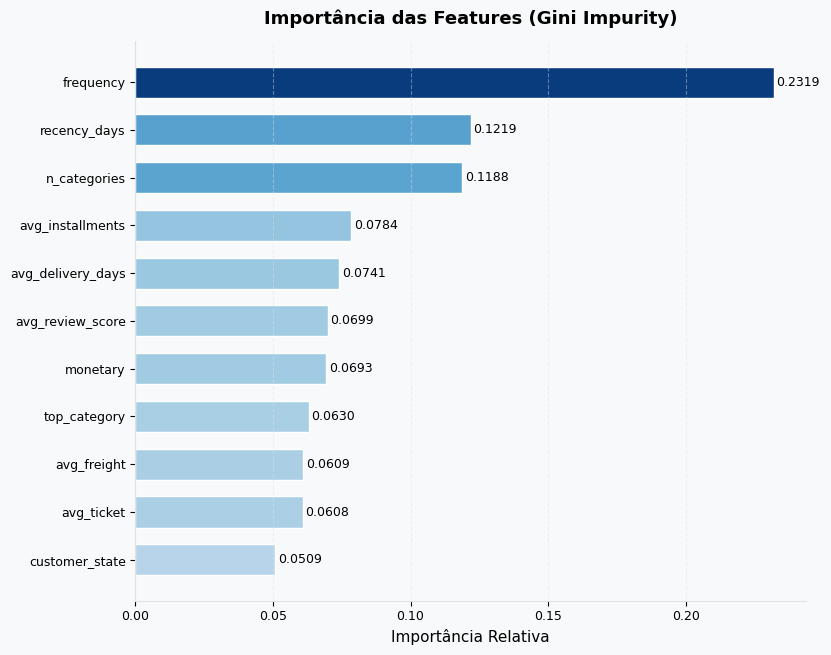
\includegraphics[width=0.9\textwidth]{USPSC-img/figuras/fig11-importancia-gini.png}
\end{center}
\begin{flushleft}
	\ABNTEXfontereduzida
	\SingleSpacing
	Fonte: elaborado pelo autor.
\end{flushleft}
\end{figure}

\begin{figure}[htbp]
\caption{Top-5 Features por impureza de Gini (Random Forest)}
\label{fig:top5-gini}
\begin{center}
	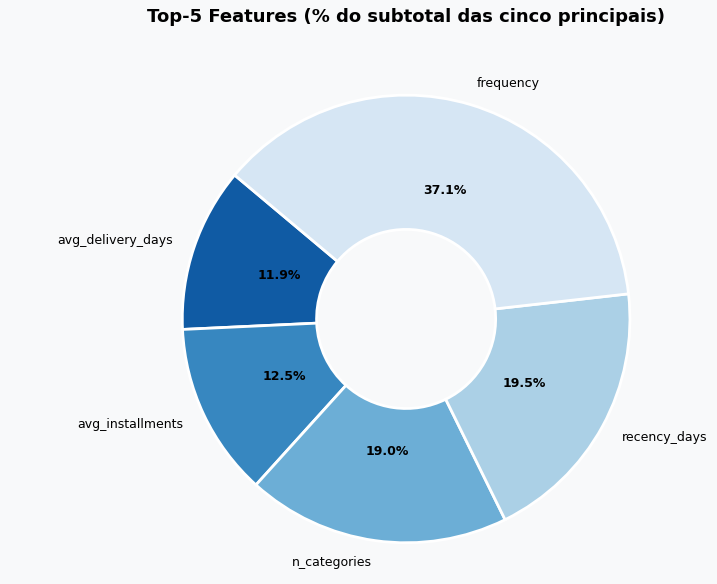
\includegraphics[width=0.85\textwidth]{USPSC-img/figuras/fig12-top5-gini.png}
\end{center}
\begin{flushleft}
	\ABNTEXfontereduzida
	\SingleSpacing
	Fonte: elaborado pelo autor.
\end{flushleft}
\end{figure}

A análise SHAP via TreeExplainer \cite{lundberg2020} enriquece o ranking de Gini ao revelar as direções dos efeitos (Figura \ref{fig:shap-beeswarm}). A Figura \ref{fig:shap-importancia} apresenta a importância média absoluta dos valores SHAP, cuja ordenação pode ser confrontada diretamente com a da Figura \ref{fig:importancia-gini}. A concordância entre os dois métodos é elevada: as quatro features mais relevantes ocupam posições idênticas em ambos os rankings, com divergência superior a uma posição em apenas duas das onze variáveis. Cabe registrar, contudo, que essa concordância não constitui validação independente da hierarquia de importância. A importância por impureza de Gini quantifica a redução de impureza produzida por cada variável nas árvores ajustadas, e o TreeSHAP percorre exatamente essas mesmas árvores para decompor as predições: ambos os estimadores derivam da mesma estrutura de modelo, de modo que sua concordância é esperada por construção. A evidência de estabilidade adotada neste trabalho é de outra natureza e apresenta-se a seguir. O valor base do modelo, $\mathbb{E}[f(x)] = 0{,}504$, reflete o balanceamento aplicado ao conjunto de treino, conforme discutido na Seção \ref{sec:limiar}.

\begin{figure}[htbp]
\caption{Importância média \shapabs{} das features (Random Forest)}
\label{fig:shap-importancia}
\begin{center}
	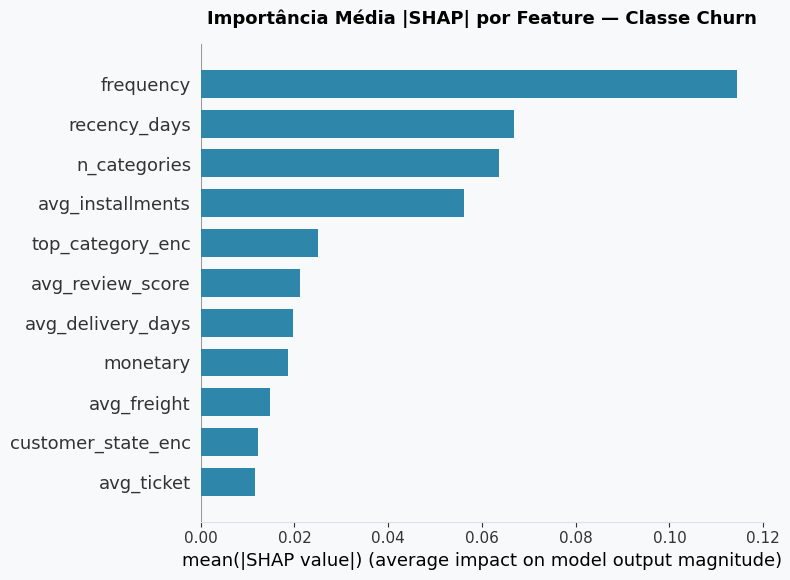
\includegraphics[width=0.9\textwidth]{USPSC-img/figuras/fig13-shap-importancia-media.png}
\end{center}
\begin{flushleft}
	\ABNTEXfontereduzida
	\SingleSpacing
	Fonte: elaborado pelo autor.
\end{flushleft}
\end{figure}

Para verificar a estabilidade da ordenação por critério independente do estimador, o modelo foi reajustado em trinta partições estratificadas independentes, registrando-se a posição de cada feature no ranking de importância por Gini em cada uma delas. A variável frequency ocupou a primeira posição nas trinta partições, sem exceção. A variável n\_categories permaneceu entre as três primeiras em 29 das trinta, com posições variando entre a segunda e a quarta, e recency\_days em 22 das trinta, com posições entre a segunda e a quinta. A variável seguinte em estabilidade, monetary, figurou entre as três primeiras em apenas quatro partições, o que delimita com clareza o trio dominante. Esse resultado sustenta a afirmação de estabilidade da hierarquia entre partições e, adicionalmente, confirma o empate técnico entre recency\_days e n\_categories registrado na Tabela \ref{tab:importancia-gini}: embora a recência esteja 0,3 ponto percentual à frente na partição de referência, a diversidade de categorias apresenta posição média superior no conjunto das trinta partições (2,30 contra 3,17).

Registra-se, por completude, que um terceiro estimador de importância, a permutação de features calculada sobre o conjunto de teste, produz ordenação distinta das duas anteriores, elevando avg\_installments à primeira posição e deslocando frequency para a quarta. Esse estimador não é informativo no regime amostral deste trabalho: com dez instâncias da classe Ativo no hold-out, o desvio-padrão de cada estimativa situa-se entre 44\% e 93\% da respectiva média nas nove variáveis de média positiva, e as duas restantes apresentam média negativa, valor que não admite interpretação substantiva. A imprecisão é suficiente para dissolver a própria ordenação que o estimador produz: a primeira e a segunda colocadas, avg\_installments (0,0788 $\pm$ 0,0449) e recency\_days (0,0721 $\pm$ 0,0508), apresentam intervalos amplamente sobrepostos. A divergência observada não refuta, portanto, a ordenação por Gini, mas impede que se afirme robustez da hierarquia ao método de estimação, razão pela qual a estabilidade entre partições foi adotada como evidência.

A análise de interpretabilidade conduzida até aqui apoia-se no Random Forest, modelo de produção. Cabe verificar em que medida a hierarquia de importância obtida é propriedade dos dados ou artefato do estimador escolhido. A importância por impureza de Gini não permite essa verificação, por não estar disponível no HistGradientBoostingClassifier nem se aplicar a modelos lineares. Os valores SHAP, ao contrário, são calculáveis para os três modelos e constituem, portanto, o único terreno comum de comparação. A Tabela \ref{tab:shap-tres-modelos} apresenta a posição de cada feature no ranking por importância média absoluta e sua participação relativa no total de cada modelo, calculadas sobre o mesmo conjunto de teste.

\begin{table}[htbp]
\ABNTEXfontereduzida
\SingleSpacing
\caption{Posição e participação relativa das features no ranking por importância média \shapabs{} nos três modelos}
\label{tab:shap-tres-modelos}
\centering
\begin{tabular}{@{}lcccrrr@{}}
\hline
\textbf{Feature} & \textbf{Pos. RF} & \textbf{Pos. HistGB} & \textbf{Pos. RL} & \textbf{\% RF} & \textbf{\% HistGB} & \textbf{\% RL} \\
\hline
frequency          & 1\textsuperscript{a}  & 1\textsuperscript{a}  & 3\textsuperscript{a}  & 27,0 & 19,4 & 13,9 \\
recency\_days      & 2\textsuperscript{a}  & 2\textsuperscript{a}  & 2\textsuperscript{a}  & 15,7 & 13,4 & 19,0 \\
n\_categories      & 3\textsuperscript{a}  & 6\textsuperscript{a}  & 4\textsuperscript{a}  & 15,0 & 8,2  & 10,6 \\
avg\_installments  & 4\textsuperscript{a}  & 4\textsuperscript{a}  & 1\textsuperscript{a}  & 13,2 & 11,7 & 21,0 \\
top\_category      & 5\textsuperscript{a}  & 5\textsuperscript{a}  & 7\textsuperscript{a}  & 5,9  & 9,5  & 6,1 \\
avg\_review\_score & 6\textsuperscript{a}  & 9\textsuperscript{a}  & 8\textsuperscript{a}  & 5,0  & 4,9  & 5,8 \\
avg\_delivery\_days& 7\textsuperscript{a}  & 3\textsuperscript{a}  & 6\textsuperscript{a}  & 4,7  & 11,8 & 6,4 \\
monetary           & 8\textsuperscript{a}  & 7\textsuperscript{a}  & 9\textsuperscript{a}  & 4,4  & 6,4  & 4,7 \\
avg\_freight       & 9\textsuperscript{a}  & 11\textsuperscript{a} & 11\textsuperscript{a} & 3,5  & 4,3  & 2,5 \\
customer\_state    & 10\textsuperscript{a} & 8\textsuperscript{a}  & 10\textsuperscript{a} & 2,9  & 5,9  & 3,7 \\
avg\_ticket        & 11\textsuperscript{a} & 10\textsuperscript{a} & 5\textsuperscript{a}  & 2,7  & 4,6  & 6,4 \\
\hline
\end{tabular}
\begin{flushleft}
	\ABNTEXfontereduzida
	\SingleSpacing
	Fonte: elaborado pelo autor.

	\textit{Nota: RF designa o Random Forest, HistGB o HistGradient Boosting e RL a Regressão Logística. Os valores absolutos de \shapabs{} não são comparáveis entre modelos e por isso não são reportados: o TreeExplainer aplicado ao Random Forest devolve contribuições em espaço de probabilidade, ao passo que o HistGradient Boosting e a Regressão Logística as devolvem em log-odds. São comparáveis a posição no ranking e a participação relativa, esta definida como a importância média absoluta da feature dividida pela soma das importâncias das onze features do mesmo modelo. Para a Regressão Logística os valores foram obtidos por LinearExplainer, que sob independência de features corresponde à forma fechada apresentada na Seção \ref{sec:shap-teorico}. Conjunto de teste, n = 236.}
\end{flushleft}
\end{table}

A convergência entre os três estimadores é substancial e estatisticamente significativa: a correlação de Spearman entre os rankings é de 0,800 entre Random Forest e HistGradient Boosting (p = 0,003) e de 0,709 nos dois pares que envolvem a Regressão Logística (p = 0,015). A recência ocupa a segunda posição nos três modelos, sem exceção, o que a torna o achado mais robusto da análise de interpretabilidade. A frequência lidera nos dois modelos baseados em árvores e cai para a terceira posição no modelo linear, resultado coerente com a natureza da relação: o beeswarm plot evidencia que o efeito da frequência é essencialmente descontínuo, concentrado na diferença entre dois pedidos e mais de dois, padrão que um modelo linear captura apenas parcialmente.

Registram-se duas divergências relevantes. A primeira é a variável avg\_installments, que ocupa a primeira posição na Regressão Logística e a quarta nos dois ensembles; sua elevação também havia sido observada pela importância por permutação, o que constitui indício independente de que seu peso é subestimado pelo Gini, ainda que aquele estimador não seja informativo neste regime amostral. A segunda é avg\_delivery\_days, terceira no HistGradient Boosting e sétima no Random Forest, deslocamento que sugere sensibilidade do algoritmo de boosting a limiares do tempo de entrega não capturados pelo ensemble por bagging. A variável n\_categories, terceira no Random Forest e quarta na Regressão Logística, cai para a sexta posição no HistGradient Boosting, de modo que a composição do trio dominante identificada nesta seção é confirmada por dois dos três estimadores, e não pelos três.

O beeswarm plot evidencia que valores baixos de frequency (poucos pedidos) aumentam significativamente a probabilidade predita de churn, enquanto valores altos a reduzem, relação capturada por uma correlação de $-0{,}862$ entre o valor da feature e sua contribuição SHAP. Para n\_categories, o padrão é análogo (correlação de $-0{,}648$): clientes com maior diversidade de categorias apresentam contribuições SHAP negativas para o churn, ou seja, a diversidade reduz o risco predito. Para recency\_days, a direção é a esperada e a associação é a mais forte entre as três (correlação de $+0{,}895$): maior recência eleva o risco de churn. Os dependence plots e os waterfall plots de instâncias representativas, apresentados ao final desta seção, detalham respectivamente os limiares não lineares dessas relações e a decomposição individual da predição para clientes típicos de cada classe.

Registra-se, como divergência pontual entre os métodos, que a variável top\_category ocupa a quinta posição no ranking SHAP, três posições acima do observado pela impureza de Gini. Esse deslocamento sugere que a categoria dominante de compra exerce efeito direcional mais relevante do que a redução de impureza isoladamente permite inferir, achado consistente com a limitação conhecida da importância por Gini em variáveis categóricas de cardinalidade elevada.

\begin{figure}[htbp]
\caption{Valores SHAP (beeswarm) das features no conjunto de teste}
\label{fig:shap-beeswarm}
\begin{center}
	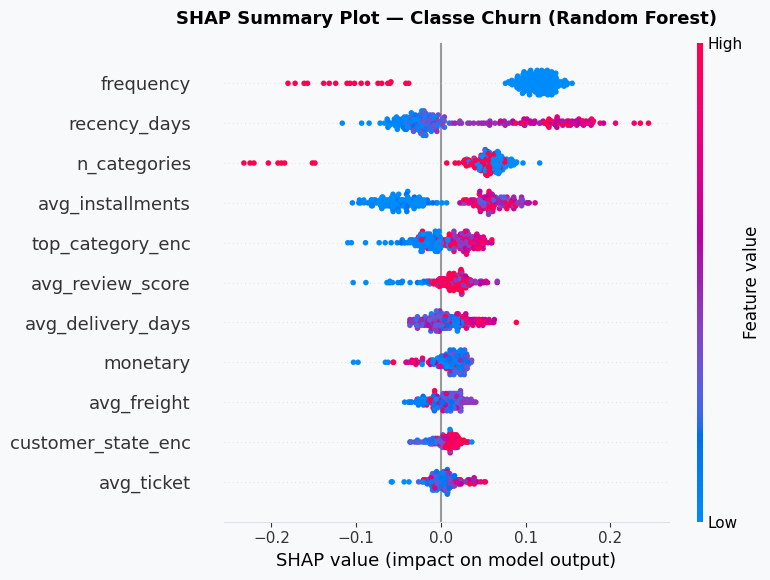
\includegraphics[width=0.9\textwidth]{USPSC-img/figuras/fig14-shap-beeswarm.png}
\end{center}
\begin{flushleft}
	\ABNTEXfontereduzida
	\SingleSpacing
	Fonte: elaborado pelo autor.
\end{flushleft}
\end{figure}

\subsection{Perfil do cliente que retorna: leitura sob a ótica da retenção} \label{subsec:perfil-retorna}

Embora a variável-alvo seja formalmente o churn, os valores SHAP permitem inverter a leitura e caracterizar diretamente o perfil do cliente que volta a comprar, objetivo de maior valor acionável para a organização. As contribuições SHAP que reduzem a probabilidade de churn correspondem, por complementaridade, aos atributos associados à retenção. Sob essa ótica, o cliente com maior propensão a retornar à plataforma apresenta o seguinte perfil: (i) realiza compras com maior frequência (2,56 pedidos em média, contra 2,08 entre os clientes Churn, conforme a Seção \ref{sec:eda}); (ii) mantém recência baixa, com intervalos curtos entre transações; e (iii) compra em mais categorias distintas (n\_categories elevado), indicando exploração ampla do catálogo. Em contraste, o uso de parcelamento em mais vezes (avg\_installments elevado) associa-se a maior risco de churn, possivelmente por sinalizar compras pontuais de maior ticket em vez de um relacionamento recorrente com a loja. Cabe observar que essa última variável é a que ocupa a primeira posição no ranking SHAP da Regressão Logística (Tabela \ref{tab:shap-tres-modelos}), o que sugere que seu efeito seja predominantemente monotônico e, por isso, mais bem capturado por um modelo linear.

Esse achado tem implicação estratégica direta: a diversidade de categorias, um dos três principais drivers do modelo, sugere que estimular o cliente a explorar novas categorias, via recomendação e cross-selling, é mecanismo promissor para elevar a probabilidade de retorno \cite{kotler2016}. A análise exploratória (Seção \ref{sec:eda}) corrobora esse perfil ao mostrar que clientes Ativos apresentam maior valor monetário acumulado (R\$ 372,25 contra R\$ 299,12) e compram em categorias mais variadas (1,80 contra 1,54 categorias, em média) que os clientes Churn. Cabe observar que o valor monetário acumulado, embora discrimine as classes na análise exploratória, ocupa apenas a sétima posição na importância por impureza de Gini, o que sugere que seu poder preditivo é em parte absorvido pela frequência de compras, com a qual mantém dependência direta.

Registra-se, como ressalva metodológica, que a classe Ativo conta com aproximadamente 50 clientes na base completa, de modo que o perfil de retenção descrito, ainda que consistente entre a análise exploratória, a importância por Gini estimada em trinta partições e os valores SHAP dos três modelos, deve ser interpretado como hipótese robusta a ser confirmada em bases de maior volume.

Todos os valores das figuras abaixo referem-se ao modelo Random Forest adotado como modelo de produção, calculados sobre o conjunto de teste. Os dependence plots das Figuras \ref{fig:dep-frequency}, \ref{fig:dep-recency} e \ref{fig:dep-ncategories} evidenciam que as relações capturadas pelo modelo não são lineares. Para frequency, as contribuições concentram-se em dois agrupamentos disjuntos: clientes com dois pedidos recebem contribuição positiva para o churn, entre 0,08 e 0,15, e clientes com três ou mais pedidos recebem contribuição negativa, o que caracteriza um limiar de decisão e não uma tendência gradual. Para recency\_days a relação é monotônica crescente e aproximadamente sigmóide, com a transição de contribuição negativa para positiva ocorrendo em torno da média da distribuição padronizada. Para n\_categories o padrão repete a descontinuidade observada em frequency, com separação nítida entre clientes de uma ou duas categorias e clientes de três ou mais. Essa descontinuidade é a razão estrutural pela qual a frequência perde posições no ranking SHAP da Regressão Logística (Tabela \ref{tab:shap-tres-modelos}): um modelo linear não representa limiares dessa natureza.

\begin{figure}[H]
\caption{Dependence plots da feature frequency no SHAP (Random Forest)}
\label{fig:dep-frequency}
\begin{center}
	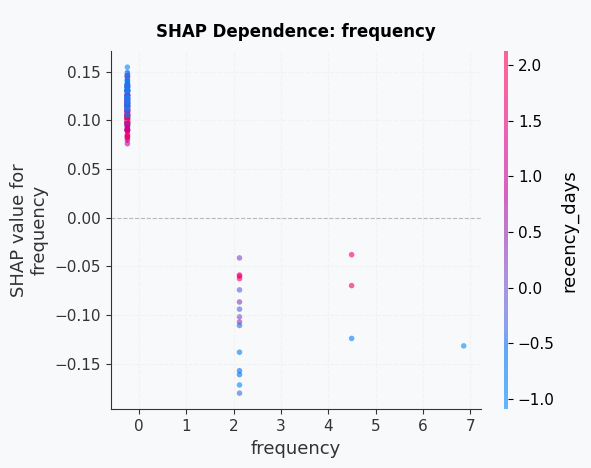
\includegraphics[width=0.80\textwidth]{USPSC-img/figuras/fig15-shap-dependence-frequency.png}
\end{center}
\begin{flushleft}
	\ABNTEXfontereduzida
	\SingleSpacing
	Fonte: elaborado pelo autor.
\end{flushleft}
\end{figure}

\begin{figure}[H]
\caption{Dependence plots da feature recency\_days no SHAP (Random Forest)}
\label{fig:dep-recency}
\begin{center}
	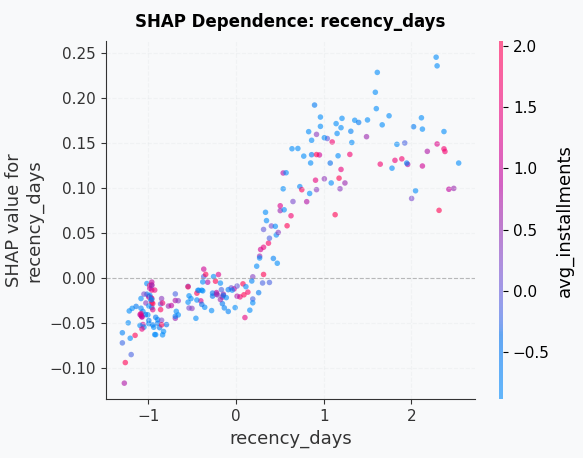
\includegraphics[width=0.85\textwidth]{USPSC-img/figuras/fig16-shap-dependence-recency.png}
\end{center}
\begin{flushleft}
	\ABNTEXfontereduzida
	\SingleSpacing
	Fonte: elaborado pelo autor.
\end{flushleft}
\end{figure}

\begin{figure}[H]
\caption{Dependence plots da feature n\_categories no SHAP (Random Forest)}
\label{fig:dep-ncategories}
\begin{center}
	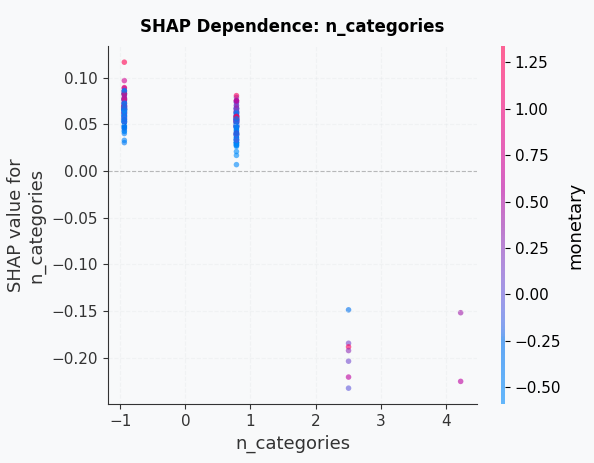
\includegraphics[width=0.85\textwidth]{USPSC-img/figuras/fig17-shap-dependence-ncategories.png}
\end{center}
\begin{flushleft}
	\ABNTEXfontereduzida
	\SingleSpacing
	Fonte: elaborado pelo autor.
\end{flushleft}
\end{figure}

As Figuras \ref{fig:waterfall-ativo} e \ref{fig:waterfall-churn} decompõem a predição individual dos clientes mais próximos do centroide de cada classe no espaço de features padronizado. Ambas partem do mesmo valor base, $\mathbb{E}[f(x)] = 0{,}504$, que reflete o balanceamento aplicado ao conjunto de treino conforme a Seção \ref{sec:limiar}.

O cliente representativo da classe Churn (Figura \ref{fig:waterfall-churn}) recebe $f(x) = 0{,}841$, valor consistente com sua classe real. A decomposição atribui o deslocamento principalmente à frequência ($+0{,}12$), à diversidade de categorias ($+0{,}08$) e ao parcelamento médio ($+0{,}07$), reproduzindo em nível individual a hierarquia agregada da Figura \ref{fig:shap-importancia}.

O cliente representativo da classe Ativo (Figura \ref{fig:waterfall-ativo}) recebe $f(x) = 0{,}613$, valor acima do limiar de 0,38 e que, portanto, o classifica incorretamente como Churn. Longe de invalidar a ilustração, esse resultado a torna mais informativa: o cliente mais próximo do centroide da classe Ativo apresenta frequência e diversidade de categorias abaixo da média da base, atributos que o modelo associa ao abandono, e as contribuições que o afastam do churn, o parcelamento médio ($-0{,}06$) e a recência ($-0{,}03$), são insuficientes para compensá-los. A figura expõe, em um caso concreto, a razão do Recall de 0,20 na classe Ativo reportado na Tabela \ref{tab:benchmark}: o perfil médio do cliente que retorna não é suficientemente distinto do perfil do cliente que abandona, limitação devida ao tamanho reduzido da classe minoritária e não à especificação do modelo. Esse é também o fundamento do critério de seleção adotado na Seção \ref{sec:benchmark}: uma vez que a decisão binária no limiar é estruturalmente limitada por esse regime amostral, o valor operacional do modelo reside na ordenação que ele produz, e não na classificação que dela resulta.

\begin{figure}[htbp]
\caption{Decomposição SHAP da predição para o cliente mais próximo do centroide da classe Ativo}
\label{fig:waterfall-ativo}
\begin{center}
	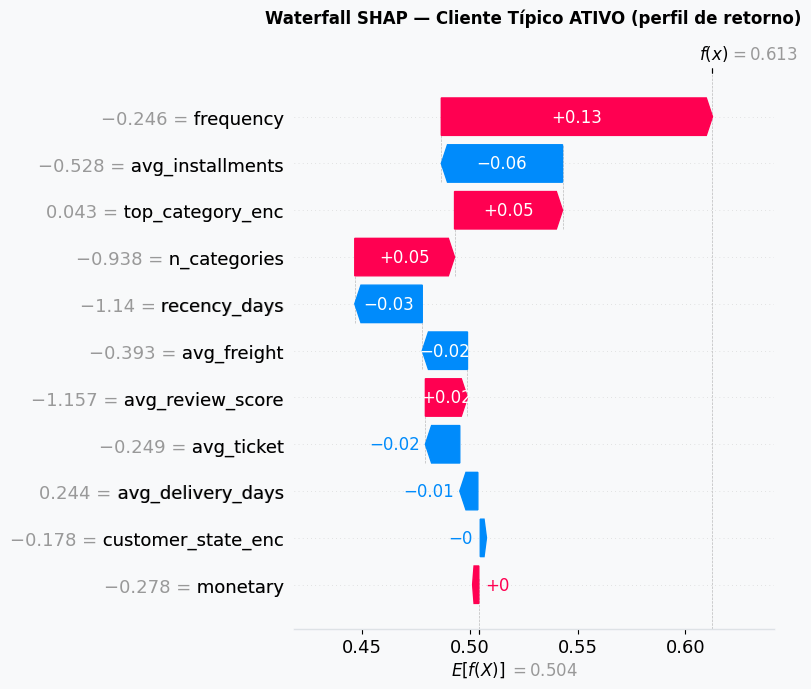
\includegraphics[width=0.9\textwidth]{USPSC-img/figuras/fig18-shap-waterfall-ativo.png}
\end{center}
\begin{flushleft}
	\ABNTEXfontereduzida
	\SingleSpacing
	Fonte: elaborado pelo autor.
\end{flushleft}
\end{figure}

\begin{figure}[htbp]
\caption{Decomposição SHAP da predição para o cliente mais próximo do centroide da classe Churn}
\label{fig:waterfall-churn}
\begin{center}
	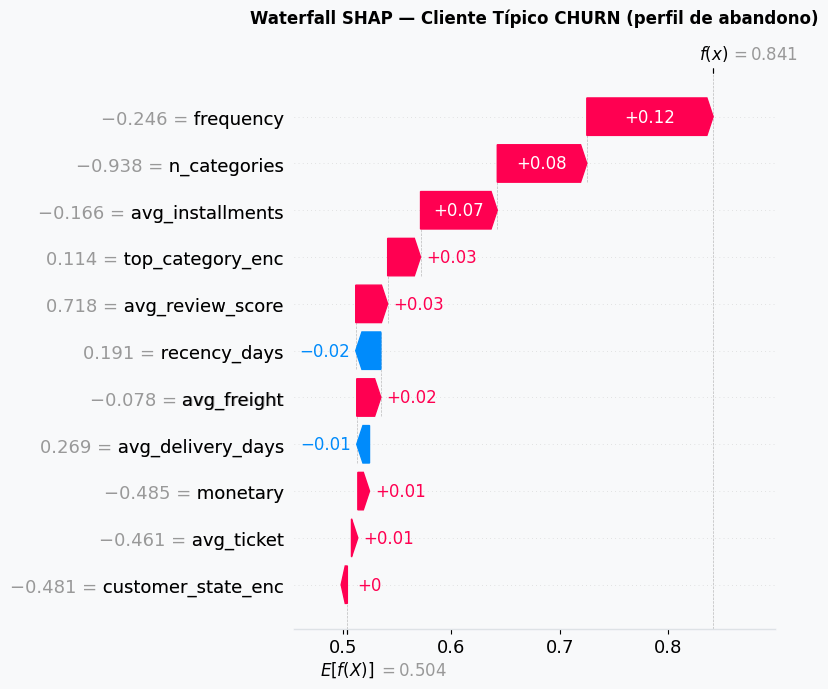
\includegraphics[width=0.9\textwidth]{USPSC-img/figuras/fig19-shap-waterfall-churn.png}
\end{center}
\begin{flushleft}
	\ABNTEXfontereduzida
	\SingleSpacing
	Fonte: elaborado pelo autor.
\end{flushleft}
\end{figure}

\FloatBarrier
\section{Segmentação de Risco e Recomendações de Negócio} \label{sec:segmentacao}

Aplicado o modelo Random Forest à base completa de 1.178 clientes, cada cliente recebeu um score de probabilidade de churn, utilizado para classificação em quatro segmentos de risco \cite{kotler2016}. Os limiares de 25\%, 50\% e 75\% que delimitam os segmentos são cortes nominais da escala de probabilidade, adotados por interpretabilidade e não otimizados sobre os dados; sua adequação é aferida a posteriori pela taxa de churn observada em cada faixa. A Figura \ref{fig:distribuicao-scores} apresenta a distribuição desses scores nos três modelos de melhor desempenho, com os limiares que delimitam os quatro segmentos, e a Tabela \ref{tab:segmentacao} detalha a distribuição e o perfil médio de cada segmento sob o modelo de produção.

\begin{figure}[htbp]
\caption{Distribuição dos scores de probabilidade de churn e limiares de segmentação nos três modelos}
\label{fig:distribuicao-scores}
\begin{center}
	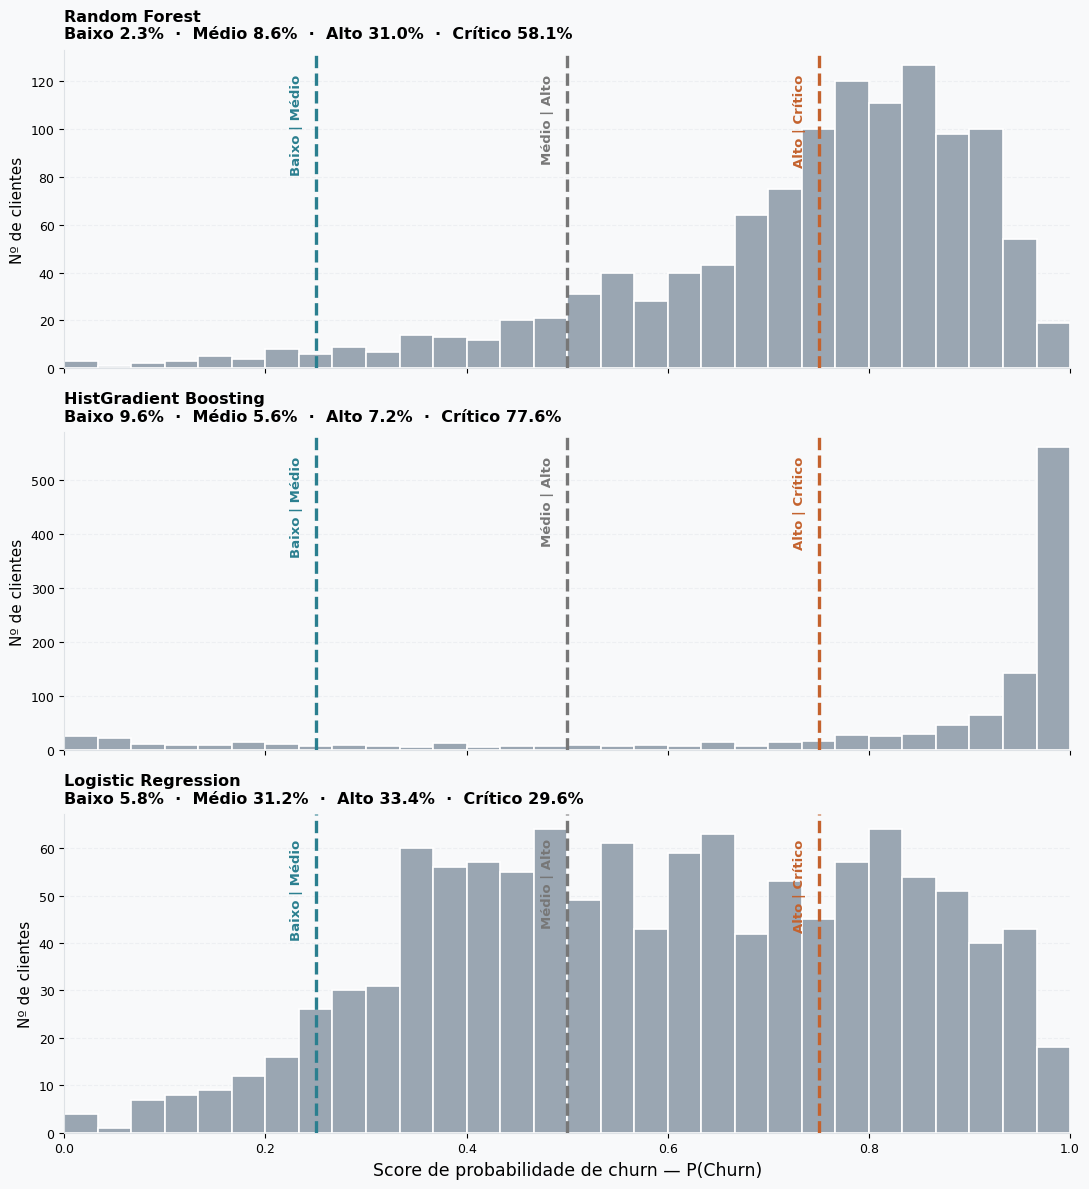
\includegraphics[width=0.95\textwidth]{USPSC-img/figuras/fig20-distribuicao-scores.png}
\end{center}
\begin{flushleft}
	\ABNTEXfontereduzida
	\SingleSpacing
	Fonte: elaborado pelo autor.

	\textit{Nota: os três painéis aplicam os mesmos cortes nominais de 25\%, 50\% e 75\%, que delimitam os segmentos de risco e não correspondem ao limiar de classificação de cada modelo (0,38 no Random Forest, 0,18 no HistGradient Boosting e 0,12 na Regressão Logística, conforme a Tabela \ref{tab:benchmark}). Os cortes de segmentação são uma escolha de negócio, aferida a posteriori pela taxa de churn observada em cada faixa; o limiar de classificação é parâmetro da regra de decisão binária, derivado das probabilidades out-of-fold conforme a Seção \ref{sec:protocolo}. Escopo: base completa de 1.178 clientes.}
\end{flushleft}
\end{figure}

\begin{table}[htbp]
\ABNTEXfontereduzida
\SingleSpacing
\caption{Segmentação de risco de churn e ações recomendadas por segmento}
\label{tab:segmentacao}
\centering
\setlength{\tabcolsep}{4pt}
\begin{tabular}{@{}l c r r >{\raggedright\arraybackslash}p{4.7cm}@{}}
\hline
\textbf{Segmento} & \textbf{Critério} & \textbf{Clientes} & \shortstack[r]{\textbf{Recência}\\\textbf{Média}} & \textbf{Ação Recomendada} \\
\hline
Crítico & $P > 75\%$              & 685 (58,1\%) & 147,95 dias & Ação urgente: cupons e contato direto \\
Alto    & $50\% < P \leq 75\%$    & 365 (31,0\%) & 95,78 dias  & Ofertas e descontos personalizados \\
Médio   & $25\% < P \leq 50\%$    & 101 (8,6\%)  & 80,72 dias  & Campanhas de reengajamento leve \\
Baixo   & $P \leq 25\%$           & 27 (2,3\%)   & 72,52 dias  & Cross-sell e manutenção de engajamento \\
\hline
\end{tabular}
\begin{flushleft}
	\ABNTEXfontereduzida
	\SingleSpacing
	Fonte: elaborado pelo autor.
\end{flushleft}
\end{table}

A validade da segmentação é aferida pela taxa de churn efetivamente observada em cada faixa, isto é, pelo próprio rótulo que o modelo busca prever, e não por variáveis que integram seu conjunto de entrada. Cabe, antes, uma delimitação de escopo: a Tabela \ref{tab:segmentacao} descreve a base completa de 1.178 clientes, que inclui as observações utilizadas no ajuste do modelo, de modo que suas contagens refletem, em parte, o comportamento do classificador sobre dados já vistos. Sobre essa base, a taxa cresce de forma estritamente monotônica ao longo dos segmentos: 22,2\% no Baixo, 79,2\% no Médio, 98,1\% no Alto e 99,9\% no Crítico, com amplitude de 77,6 pontos percentuais entre os extremos.

A leitura com valor preditivo, contudo, é restrita ao conjunto de teste, cujos 236 clientes não participaram do ajuste. Nele, a progressão mantém-se na mesma direção (75,0\% no Baixo e 99,3\% no Crítico), com inversão entre as faixas Médio e Alto atribuível ao reduzido número de observações por segmento. Os dez clientes ativos do conjunto de teste distribuem-se em um no Baixo, um no Médio, sete no Alto e um no Crítico. O resultado operacionalmente relevante está, portanto, na exclusão da faixa Crítico: fora dela permanecem nove dos dez clientes Ativos, em 92 das 236 observações (39,0\%), o que corresponde a um lift de 2,31 vezes sobre a proporção de Ativos no conjunto de teste (4,2\%). A mesma métrica calculada sobre a base completa resulta em 2,34 vezes (49 dos 50 Ativos em 41,9\% das observações), estabilidade que indica não haver, nesse recorte, ganho atribuível à memorização das observações de treino.

Registra-se, por transparência, que o recorte alternativo composto pelas duas faixas de menor risco não apresenta a mesma estabilidade: na base completa ele reúne 42 dos 50 clientes Ativos em 10,9\% das observações, lift de 7,73 vezes, mas no conjunto de teste reúne apenas dois dos dez em 8,1\%, lift de 2,48 vezes. A diferença decorre de os quarenta clientes ativos presentes no conjunto de treino situarem-se integralmente nessas duas faixas. Verifica-se, assim, que a estratificação separa risco fora da amostra, com magnitude da ordem de duas vezes, magnitude que deve ser lida com cautela em razão do número reduzido de clientes Ativos no conjunto de teste.

Com base nos scores de risco, propõem-se ações diferenciadas de retenção: clientes no segmento Baixo devem ser priorizados para cross-sell; no Médio, são candidatos a campanhas de reengajamento leve, como newsletters; o segmento Alto requer abordagem mais ativa, com descontos personalizados; e o segmento Crítico demanda ação urgente, com cupons de alto impacto antes do abandono definitivo. O princípio econômico orientador é escalonar o investimento conforme o risco cresce, aplicação prática do argumento de \citeonline{reichheld2000} de que, no comércio eletrônico, a rentabilidade do cliente depende da extensão do relacionamento, o que torna a retenção economicamente preferível à reaquisição. A leitura em cobertura fixa apresentada na Seção \ref{sec:benchmark} fornece o parâmetro de dimensionamento dessas campanhas: abordar 35,6\% dos clientes (fração medida no conjunto de teste, único recorte fora da amostra) é suficiente, sob o modelo de produção, para alcançar 90\% dos clientes com propensão real ao retorno.

\FloatBarrier
